\documentclass[12pt,a4paper,UTF8]{article}
\usepackage[fontset=fandol]{ctex} % Chinese support, using Fandol fonts
\usepackage{graphicx} % Insert images
\usepackage{listings} % Print source code
\usepackage{xcolor} % Color support
\usepackage{booktabs} % Professional table support
\usepackage{pdflscape} % Landscape pages support in PDF
\usepackage{hyperref} % Hypertext links support for cross-referencing
\usepackage{inconsolata} % 使用 Inconsolata 等宽字体

% Customize hyperref format (it's set to no special format here)
\hypersetup{hidelinks}

% Declare directories to search for graphics files for graphicx
\graphicspath{{figures/}{logo/}}

% Define source code style for listings
% Define source code style for listings
\lstdefinestyle{c-style}{
  language=C,
  basicstyle=\ttfamily\small, % 使用等宽字体
  keywordstyle=\bfseries\color{blue},
  identifierstyle=\color{teal},
  stringstyle=\color{purple},
  commentstyle=\itshape\color{green!50!black},
  backgroundcolor=\color{gray!5},
  numbers=left,
  numbersep=8pt,
  numberstyle=\tiny\color{gray},
  breaklines=true,
  postbreak=\mbox{\textcolor{red}{$\hookrightarrow$}\space},
  frame=single,
  framerule=0.5pt,
  rulecolor=\color{black},
  tabsize=4,
  captionpos=b,
  showspaces=false,
  showstringspaces=false,
  showtabs=false,
  morekeywords={*,printf,scanf},
  escapeinside={(*@}{@*)}, % 支持代码中插入LaTeX
}

% Define new command for title page
\newcommand{\reporttitle}[2]{
  \LARGE\textsf{#1}\quad\underline{\makebox[12em]{#2}}
}
\newcommand{\reportinfo}[2]{
  \large\makebox[4em]{\textsf{#1}}\quad\underline{\makebox[18em]{#2}}
}

% ----- The document begins here -----
\begin{document}
  \begin{titlepage}
    \centering
    \vspace*{\fill}
    
\includegraphics[height=144pt]{hust_logo}\\[48pt] % School logo
    {\huge\textsf{课\ 程\ 实\ 验\ 报\ 告}}\\[52pt]
    \reporttitle{实验名称}{立扫帚实验}\\[68pt]

    \reportinfo{课程名称}{计算机}\\[8pt]
    \reportinfo{院\hspace{\fill}系}{华科计算机学院}\\[10pt]
    \reportinfo{学\hspace{\fill}号}{U202115373}\\[8pt]
    \reportinfo{学生姓名}{雷翔麟}\\[8pt]
    \reportinfo{指导教师}{赫敏·格兰杰}\\[8pt]
    \reportinfo{实验日期}{2024年8月}\\
    \vspace*{\fill}
  \end{titlepage}

  \tableofcontents

  \newpage
  \section{实验目的}
  \begin{enumerate}
    \item 学会寻找扫帚的重心,培养学生的耐心;
    \item 验证基本物理定律在霍格沃茨的有效性。
  \end{enumerate}

  \section{实验内容}
  一些麻瓜称,根据 NASA 的测算,由于天体运行导致地球的磁场和重力场发生变化,只有在2月10日当天扫帚才可以立起来。
  次日,NASA 副局长 Jim Morhard 回应称上述说法不实,基本物理定律每天都有效,并演示了这个实验,如图 \ref{JimMorhard} 所示。

  % Insert an image, with placement specifier htbp
  \begin{figure}[htbp]
    \centering
    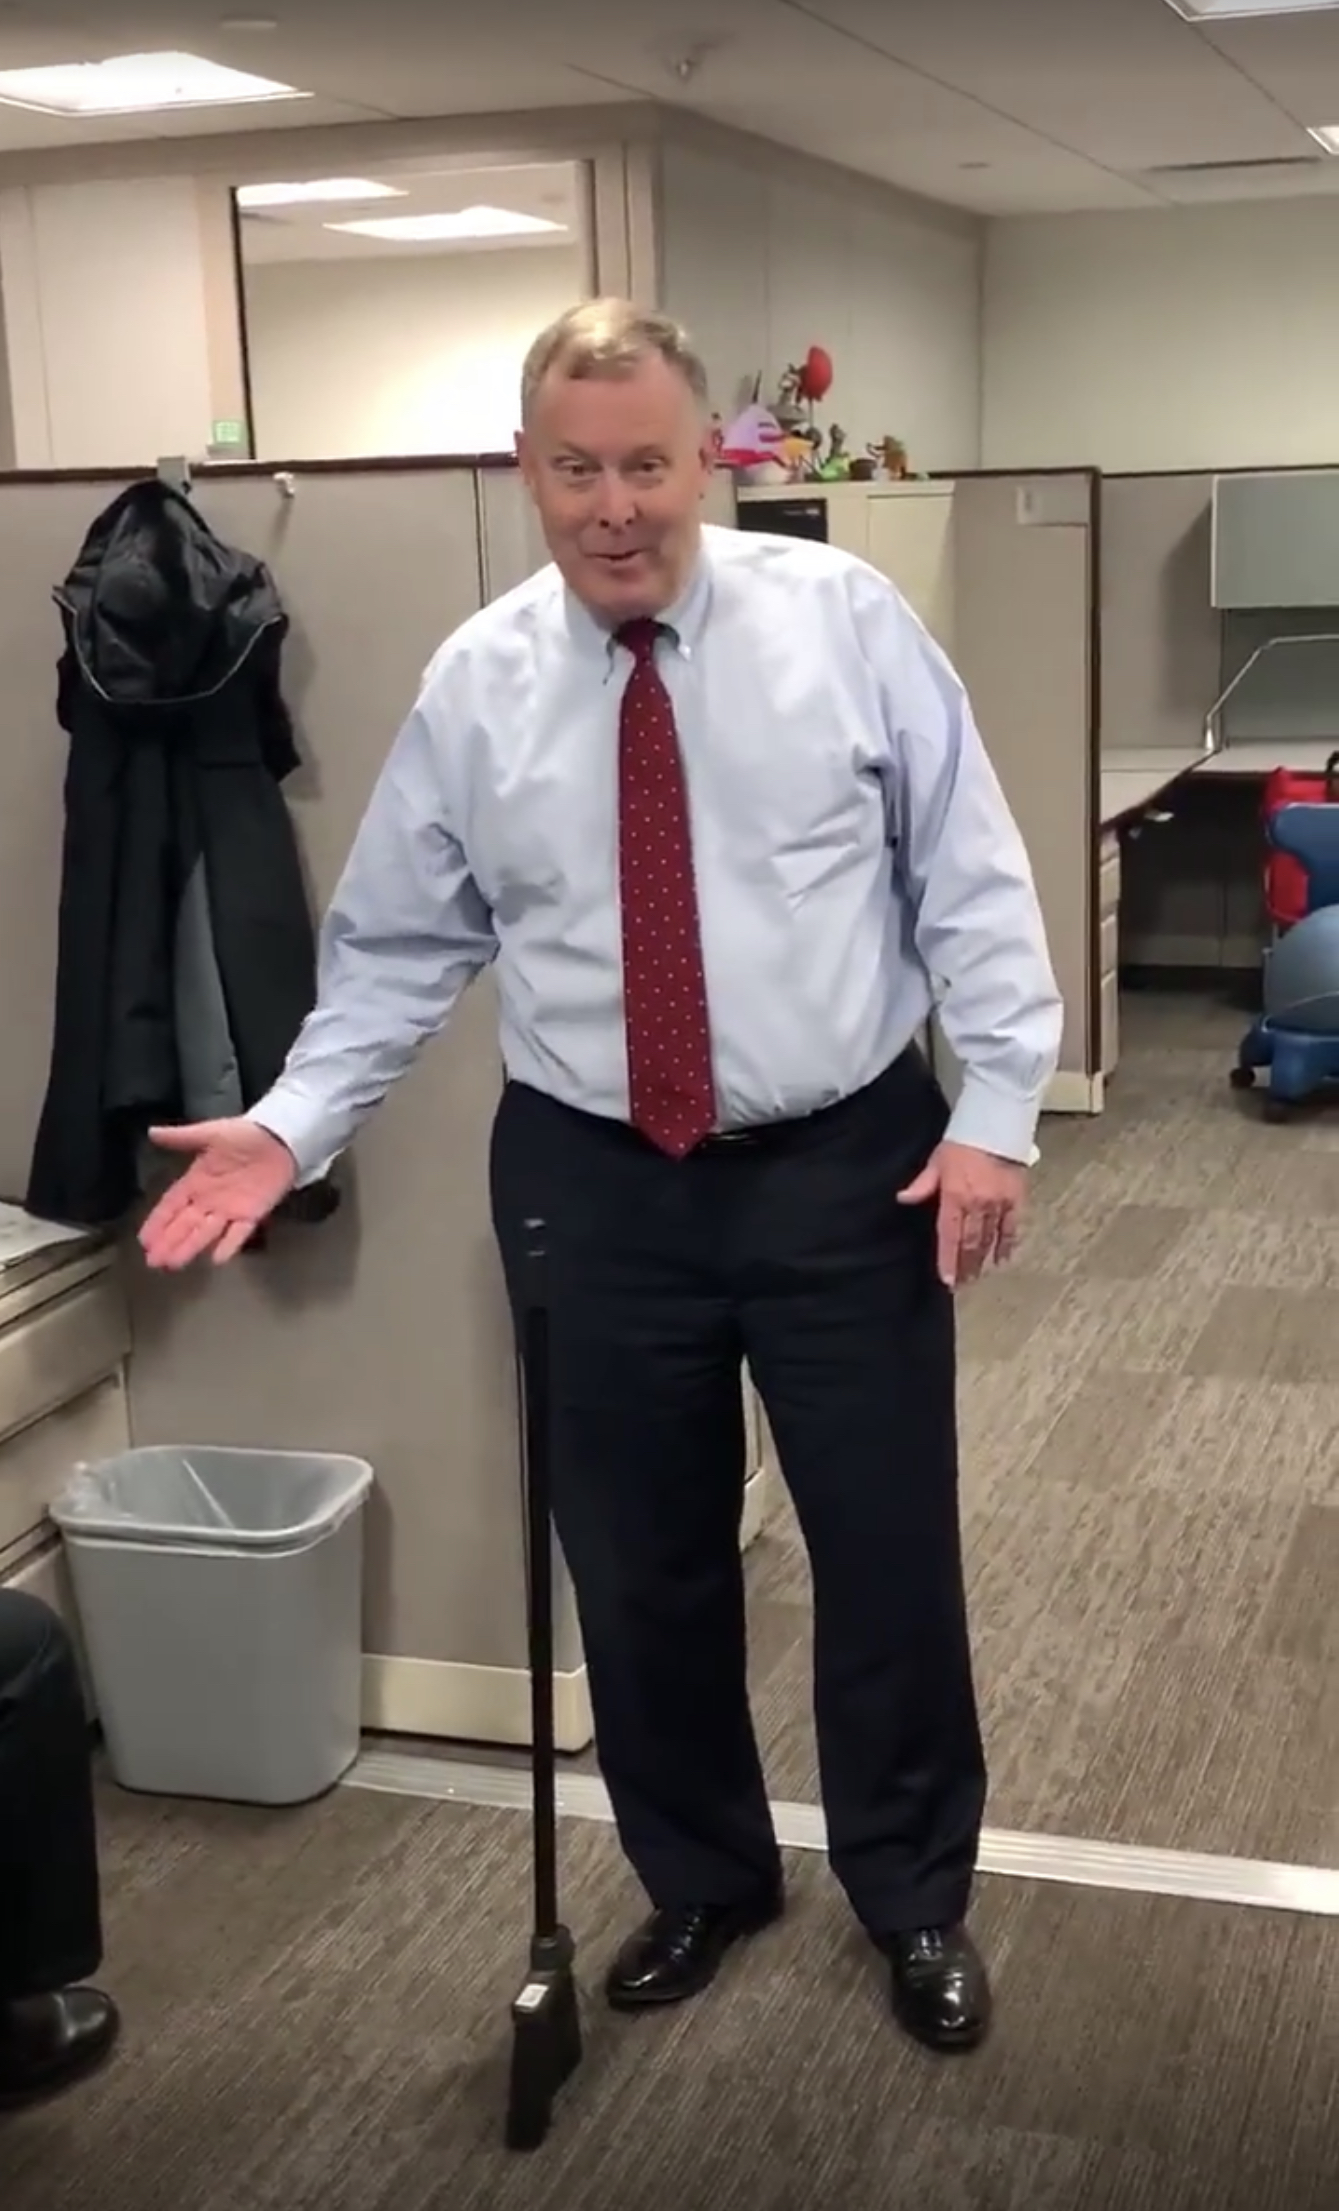
\includegraphics[width=0.5\textwidth]{JimMorhard}
    \caption{Jim Morhard 演示立扫帚实验}
    \label{JimMorhard}
  \end{figure}

  实验具体要求如下:
  \begin{enumerate}
    \item 扫帚必须能够单独站立,不可以借助其它外力;
    \item 实验过程中不得使用咒语,尤其是不得使用永久粘贴咒将扫帚粘在地上。
  \end{enumerate}

  \section{实验过程}
  \subsection{扫帚的选择}
  不同的扫帚参数各异,这里列出了部分扫帚的参数,请见表 \ref{broomsticks}。

  % Insert a three-line table
  \begin{table}[htbp]
    \centering
    \begin{tabular}{cccc}
      \toprule
      序号 & 名称 & 上市时间 & 最高时速 \\
      \midrule
      1 & 彗星290 & 1995年 & 60\,mph \\
      2 & 光轮1000 & 1967年 & 100\,mph \\
      3 & 光轮2001 & 1992年 & >\,100\,mph \\
      4 & 火弩箭 & 1993年 & 150\,mph \\
      \bottomrule
    \end{tabular}
    \caption{部分扫帚的参数对比}
    \label{broomsticks}
  \end{table}

  但是,本次实验不是魁地奇比赛,扫帚的最高时速对实验的进行没有太大的影响。
  为了选出合适的扫帚,这里采用随机抽签的办法,编写了一个 C 程序进行抽取:

  % Insert source code
  \lstinputlisting[style=c-style]{random.c}

  % Insert an image in a separate landscape page
  \begin{landscape}
    \begin{figure}
      \centering
      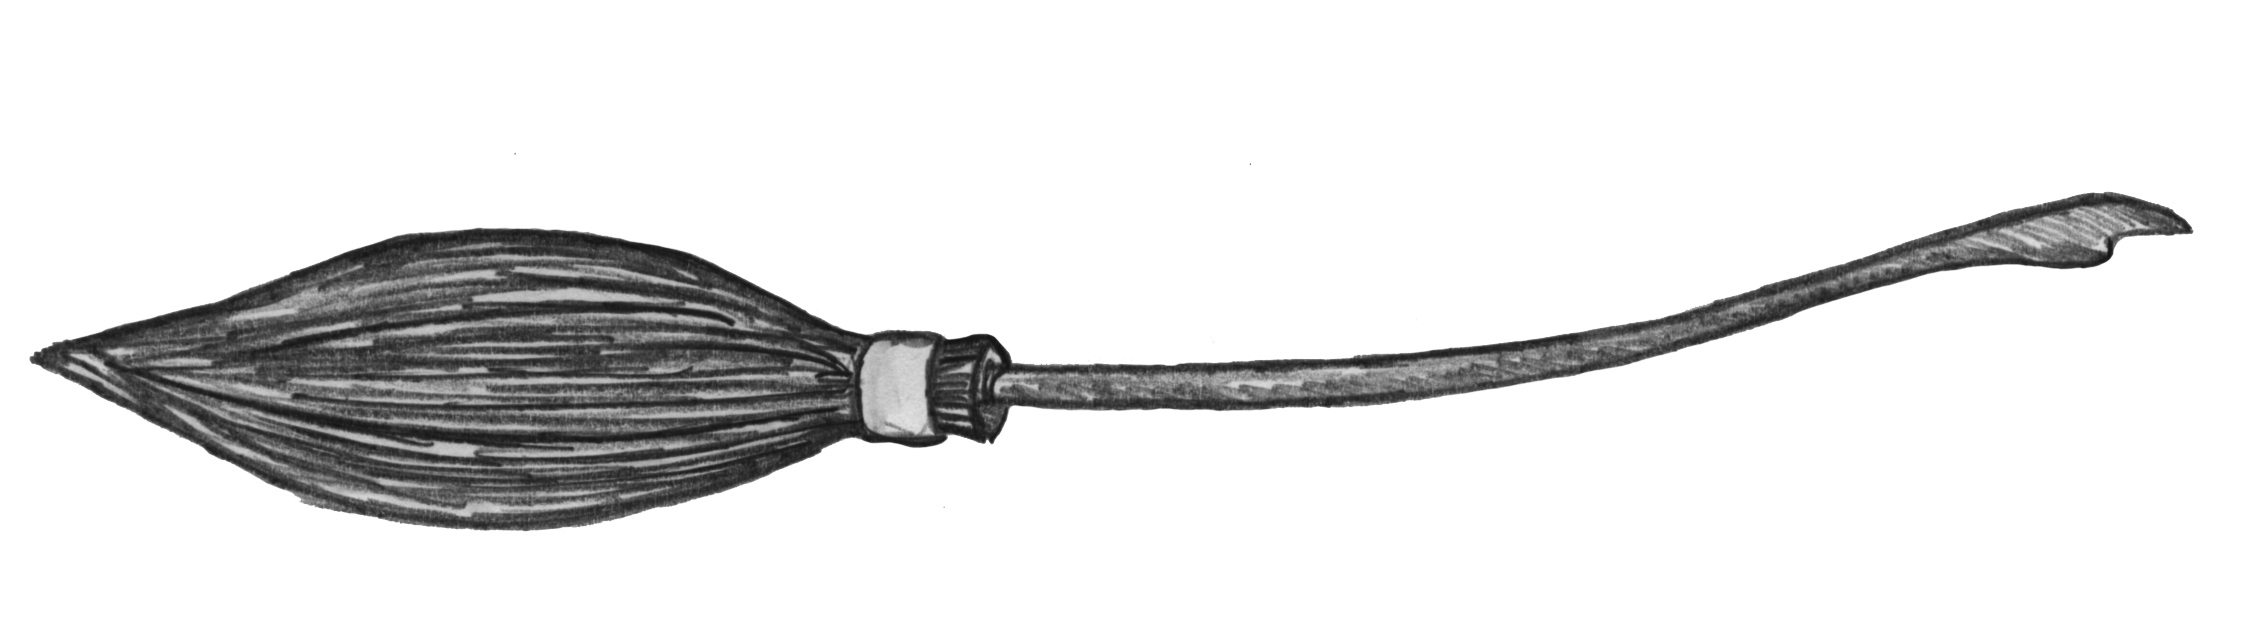
\includegraphics[width=\linewidth]{Nimbus2001}
      \caption{光轮2001扫帚}
      \label{Nimbus2001}
    \end{figure}
  \end{landscape}

  编译并运行上述程序,得到结果为 3,因此这里选择光轮 2001 扫帚进行实验。

  \subsection{扫帚起竖}
  光轮 2001 扫帚如图 \ref{Nimbus2001} 所示,与麻瓜使用的扫帚相比,有以下区别:
  \begin{enumerate}
    \item 扫帚末端较尖,同时在各个方向上都不是平面;
    \item 扫帚柄有一定弯曲,重心不易估计。
  \end{enumerate}

  为了解决上述问题,我在实验中采用了先将扫帚毛从中间稍稍分开,用手扶着竖直立在地上后,再进行调整的方式。
  调整的过程中,先将扫帚向扫帚柄弯曲的反方向旋转一定角度以抵消弯曲的扫帚柄产生的影响,之后再不断尝试进行微调。
  经过近 10 分钟的不懈努力,扫帚被成功立起。

  \section{实验总结}
  本次实验中,扫帚被成功立起,证实了在不使用魔法的情况下,基本物理定律在霍格沃茨仍然适用。
\end{document}
